\documentclass[a4paper]{article}
\usepackage{amssymb,amsmath,amsfonts}       %American Math Society packages
\usepackage{color}
\usepackage[pagebackref=true]{hyperref}     %allows back reference from bibliography entry
\hypersetup{
    pdfauthor = Derek H. Ogle,
    plainpages = false,                     %front matter pages saved as page.i instead of page.1 to reduce errors
    colorlinks = true,                      %allows colored links to be used -- rather than boxes
    linkcolor = red,                        %general internal links (to equations, tables, from TOC)
    citecolor = blue,                       %color for citations
    urlcolor = magenta,                     %color for linked URLs
    bookmarksopen = false,                  %opens bookmark tree in acrobat
    breaklinks = true                       %allows long links to break onto two lines
}
\usepackage{C:/Apps/R/R-2.6.1/share/texmf/Sweave}

%==================================================================================================================================
% Overall Style Definitions --- Sizes
%==================================================================================================================================
% These are for letter paper
  \oddsidemargin = 0in    %default is 1 in, this keeps it at 1 in
  \evensidemargin = 0in
  \textheight = 9.5in

\textwidth = 6.5in
\topmargin = 0in
\headheight = 0.2in
\headsep = 0.2in

\parskip = 0.125in
\parindent = 0.0in

\newcommand{\R}[1]{      % command to put around R functions that are within a sentence
  \texttt{#1}            % Use \R{summary(lm1)}
}

\newcommand{\var}[1]{    % command to put around data variables thatare within a sentence
  \textsf{\textsl{#1}}   % Use \var{Eggs}
}

\newcommand{\dfile}[1]{  % command to put around data file names that are within a sentence
  \textsf{#1}            % Use \dfile{Eggs}
}

%defines a figure reference command so you don't have to type Figure each time
\newcommand{\figref}[1]{
  \hspace{-0.4em}\textbf{Figure \ref{#1}}\hspace{-0.3em}
}

%same as above but automatically in parentheses
\newcommand{\figrefp}[1]{
  \hspace{-0.4em}\textbf{(Figure \ref{#1})}\hspace{-0.3em}
}

%same as \figref except for tables
\newcommand{\tabref}[1]{
  \hspace{-0.4em}\textbf{Table \ref{#1}}\hspace{-0.3em}
}

%same as \figrefp except for tables
\newcommand{\tabrefp}[1]{
  \hspace{-0.4em}\textbf{(Table \ref{#1})}\hspace{-0.3em}
}

\newcommand{\sectref}[1]{
  \hspace{-0.4em}\textbf{Section \ref{#1}}\hspace{-0.3em}
}

\newcommand{\sectrefp}[1]{
  \hspace{-0.4em}\textbf{(Section \ref{#1})}\hspace{-0.3em}
}

\newenvironment{Itemize}{
\begin{itemize}
  \setlength{\topsep}{1pt}      %doesn't seem to have an effect
  \setlength{\partopsep}{1pt}   %doesn't seem to have an effect
  \setlength{\itemsep}{1pt}
  \setlength{\parskip}{0pt}     %doesn't seem to have an effect
  \setlength{\parsep}{0pt}}     %doesn't seem to have an effect
{\end{itemize}
}

\newenvironment{Enumerate}{
\begin{enumerate}
  \setlength{\topsep}{1pt}
  \setlength{\partopsep}{1pt}
  \setlength{\itemsep}{1pt}
  \setlength{\parskip}{0pt}
  \setlength{\parsep}{0pt}}
{\end{enumerate}
} 

%removes extra space in SCHUNKs
\fvset{listparameters={\setlength{\topsep}{0pt}}}
\renewenvironment{Schunk}{\vspace{\topsep}}{\vspace{\topsep}}

\begin{document}

\title{Setup of R and Packages}
\author{Derek H. Ogle}
\date{}  % makes date blank -- title will only have the title and author above then
\maketitle

This document explains how to download and install R on your own computer; how to download, install, and load external packages; and how to download, install, and load the \R{NCStats}, \R{FSAdata}, and \R{FSA} package from the class web page.

\section{Installing R on Your Computer} \label{sect:RInstall}
The latest version of R for Windows can be downloaded from the \href{http://www.ncfaculty.net/dogle/R/R.html}{``R Resources at Northland College''} web page linked to from the \href{http://fwcb.cfans.umn.edu/courses/fisheryupdate/}{class webpage}.  More generally you can go to \href{http://www.r-project.org/index.html}{www.r-project.org/} which can be used to re-direct yourself to \href{http://cran.r-project.org/mirrors.html}{cran.r-project.org/mirrors.html} where you can choose a mirror site to download R from.  It is generally best to choose a mirror site geographically closest to your locale (the U.S. sites are at the bottom of the page).  After choosing the mirror of your choice you will be presented with a page to choose the operating system of your choice.  The description below assumes that you are using a Windows machine.  This link should result in a dialog box asking you to \verb"Run" or \verb"Save" an ``.exe'' file.  You should save this file to a temporary directory on your hard drive.

Once the file is downloaded (this may take a while as it is fairly large) you can begin the installation process by navigating to where you saved the file and then opening that file (i.e., double-clicking it).  You will immediately be asked what language to use -- the default is ``English'' so you can just press \verb"OK" on this first dialog box (unless, of course, you want to install it in a different language).  You will then be brought to a setup wizard which will lead you through the following steps
\begin{Enumerate}
  \item Press \verb"Next"
  \item Examine the license agreement, if asked then check \verb"I accept the agreement", and press \verb"Next".
  \item Select a location to install the R program.  The default is likely \verb"C:\Program Files\R\R-2.6.2" (or slightly different for newer versions) but you can choose another location by selecting the \verb"Browse" button.
  \item Select components to install.  Typically I will accept the default settings.  You may install some reference material by selecting \verb"PDF Reference Manual" although these are also available on-line.  Install the selected components by pressing \verb"Next".
  \item Do not select a customized setup by selecting \verb"No (accept defaults)" and press \verb"Next".
  \item Select a folder in the start menu for the R program and then press \verb"Next".
  \item Select additional tasks (I suggest just using the defaults) and press \verb"Next".
  \item The installer will then install the required R files (this will take 1-3 minutes depending on the speed of your computer).  Press \verb"Finish" when the installer says that R has been successfully installed.
\end{Enumerate}

If you used all of the default settings you should now have an R icon on your desktop.  You can double-click this icon to start R.


\section{Using R Packages} \label{sect:RPackages}
\subsection{Installing Packages}  \label{sect:RPkgInstall}
The R program is constantly being extended by the construction of so-called packages by users from around the world.  These packages are maintained as \verb".ZIP" files at the same CRAN mirrors where you downloaded the base R program.  The downloading and installation of these packages is made very efficient with the \verb"Packages..Install Package(s)" menu item.  The directions below will show how to download and install the \verb"car" package -- an example package that will be used later in this course.  These directions will have to be repeated if other packages are to be downloaded and installed.  Note that you need to be connected to the internet to download and install packages.

Once the \verb"Packages..Install Package(s)" menu item is selected you may be presented with a long list of possible CRAN mirror sites.  Note that you may not be presented with this list of possible mirrors on subsequent attempts to download packages (i.e., R maintains your mirror selection.  This can be modified with the \verb"Packages..Set CRAN Mirror" menu option.).  Simply select from this list the mirror location that is geographically closest to you.  Once this mirror is selected, R will make a connection to the mirror and then provide a dialog box with a very long selection of available packages (see below -- note that this list was modified to save space).

\begin{center}
  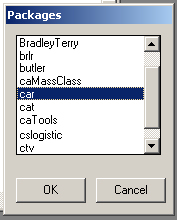
\includegraphics[width=2in]{Figs/Install_Pkg_1.jpg}
\end{center}

Select the package to be downloaded and installed from this list and then press \verb"OK".  R will then download the selected package and any dependent packages, extract them from their ZIP files, and install them into the R program.  A successful downloading and installation of the package should be noted in the R Console window (see below).

\begin{center}
  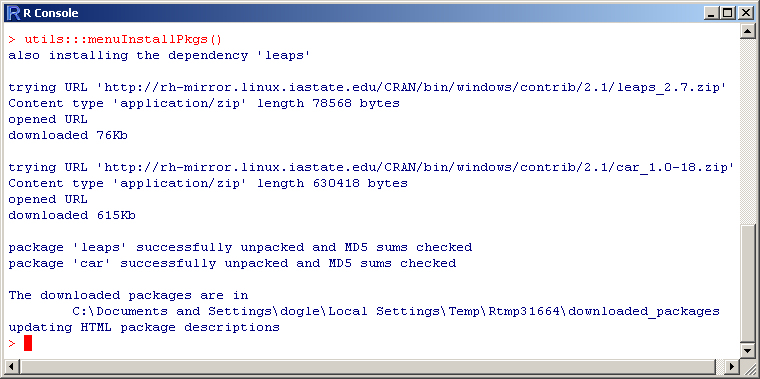
\includegraphics[width=5.5in]{Figs/Install_Pkg_2.jpg}
\end{center}

Once a package has been downloaded and installed it will not need to be installed again unless the package is updated or R has been uninstalled and then reinstalled.  In other words, the steps above do not need to be repeated in the future for any given package (however, they are repeated if different packages are to be installed).

\subsection{Loading Packages}  \label{sect:RPkgLoad}
Installed packages are not immediately available for use when you start R.  A package must be loaded into the computers memory each time you start R before the functions within the package are available for use.  Packages are loaded with the \verb"Packages..Load Package" menu item.  Once this menu item is chosen a list of packages that have been previously downloaded and installed will be shown.  Select the package to load from this list and press \verb"OK".  The functions provided by the package are then available for use in R.

Packages may also be loaded by using the \R{library()} function on the command line (how to use the command line is shown later).  The only argument to this function is the name of the package to load.  Thus, for example, the \verb"car" package can be loaded with \R{library(car)}.

The following should be noted regarding loading packages,
\begin{Itemize}
  \item Only packages that have been previously downloaded and installed (see previous section) can be loaded.
  \item A package must be loaded every time you begin a new R session.  Packages are only downloaded and installed once, but they must be loaded (into memory) every time you start a new session with R.
\end{Itemize}


\section{Using the FSA and NCStats Packages} \label{sect:NCStats}
The \R{FSA} package is a package of routines that I (DHO) have developed to perform specific fisheries-related analyses. This package relies on two other packages -- \R{FSAdata} which contains a variety of fisheries-related datasets and \R{NCStats} which is used to perform specific tasks for the statistics classes at Northland College.  None of these three packages has been developed to the point where it can be distributed internationally as the packages described in \sectref{sect:RPackages}.  Thus these packages are only available ``locally'' and, thus, the installation process is different.

Prior to installing the \R{FSA}, \R{FSAdata}, and \R{NCStats} packages you must install all packages for which these packages depend.  In other words, you must follow the directions outlined in \sectref{sect:RPkgInstall} above for each of the following packages (they can be selected all-at-once by holding down the CTRL key when selecting with the mouse),
\begin{Enumerate}
  \item car
  \item exactRankTests
  \item gplots
  \item Hmisc
  \item multcomp
  \item nortest
  \item plotrix
  \item reshape
  \item TeachingDemos
\end{Enumerate}

The steps for installing one of these local packages will be described below for the \R{NCStats} package.  This process should be repeated for the \R{FSA} and \R{FSAdata} packages.

The \R{NCStats} package can be downloaded from the class webpage through the ``R Resources at Northland College'' link.  This link leads to a page that contains, among other things, links to the three packages that I have developed.  You should download the ``Windows Binary Installation (ZIP)'' file for \R{NCStats} package by right-clicking on the provided link and saving (not opening) the linked file to a temporary folder on your hard drive.  Once downloaded, you should open R and install the \R{NCStats} package by using the \verb"Packages..Install Package from Local Zip File" menu item.  In the ensuing dialog box browse to the location of the downloaded zip file and press \verb"OK".  The \R{NCStats} package should then install without error.

Once the \R{NCStats} package is successfully installed it can be downloaded as with any other package \sectrefp{sect:RPkgLoad}.

\end{document}
